\chapter{Discussions et ouvertures}
Dans les chapitres précédents, nous avons présenté les trois outils (\gls{impatient}, \gls{nlmyo} et \gls{myoquant}) que nous avons développés pour exploiter les données multimodales de patients atteints de myopathies congénitales. Bien que ces méthodes soient fonctionnelles, elles présentent des challenges et des perspectives d'amélioration à la fois biologiques et techniques. Au niveau biologique (interprétation des résultats), nous allons discuter de l'intégration des données génomiques comme modalité supplémentaire ainsi que de la question de la mise en relation des différentes modalités entre elles (clinique, histologique et génétique). Au niveau technique, il est important d'aborder la question de l'explicabilité des systèmes \gls{ia}, des ressources nécessaires à la mise en place de systèmes \gls{ia} et des aspects législatifs de la mise en place de tels systèmes pour le traitement de données de santé. Enfin, une dernière perspective de valorisation des travaux sera abordée concernant l'intégration des outils dans un projet de création de produit combinant les outils en un seul point d'accès unique.

\section{Intégration de nouvelles modalités de données: les données génomiques}
Les outils développés se sont concentrés majoritairement sur l'exploitation des comptes rendus médicaux et des données de type imagerie. Le traitement des données génomiques dans le système \gls{impatient} est sommaire: il est possible d'associer un gène muté responsable de la maladie (et une mutation) pour un patient et de filtrer les symptômes en fonction du gène muté d'intérêt. Cependant, dans les maladies rares et génétiques, une difficulté majeure est justement de trouver la mutation causant la maladie. Pour rappel, 50\% des patients atteints de myopathies congénitales n'ont pas de diagnostic génétique à ce jour. Ainsi il serait intéressant d'ajouter au panel d'outils développés ici des outils capables d'analyser des données de séquençage pour détecter et prioriser des mutations potentiellement responsables de maladies génétiques. 

Par exemple, la figure \ref{fig:variant_discuss} présente une façon d'intégrer les données génomiques. L'utilisateur pourrait joindre au dossier du patient un fichier VCF listant les variants trouvés dans son génome. À partir de cette liste, il serait possible de filtrer les variants pour ne garder que les variants liés aux gènes des myopathies congénitales puis de classer les variants par niveau de pathogénicité (en intégrant des outils de prédiction de pathogénicité comme MISTIC (\cite{chennen_mistic_2020})). Enfin, il serait possible de prioriser les variants de cette liste en croisant la liste avec les données phénotypiques et histologiques. Par exemple dans le cadre des myopathies à némaline, la présence de bâtonnets dans les fibres musculaires est souvent liée à une mutation dans les gènes NEB, TPM2, TPM3 ou ACTA1. Ainsi on pourrait filtrer la liste de variants pour ne conserver que les variants pathogènes dans ces gènes. Cette approche pourrait permettre de filtrer rapidement de potentiels variants responsables de la maladie génétique du patient.

Cependant, la recherche exhaustive de variants génétiques par séquençage complet du génome n'est pas universellement disponible en France et donc les données sont limitées. Des initiatives comme le Plan France Médecine Génomique 2025 visent à démocratiser la médecine génomique pour le diagnostic des patients.
 \begin{figure}[!ht]
 \centering
 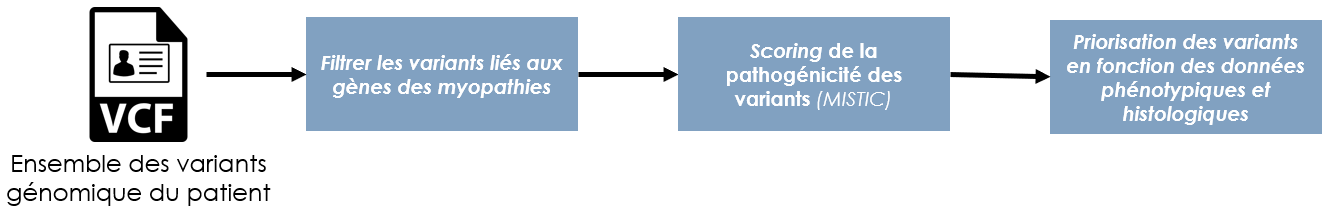
\includegraphics[width=1\textwidth]{figures/variant_discuss.png}
 \caption[Exemple de méthode d'intégration des données génomiques]{\textbf{Exemple de méthode d'intégration des données génomiques.} Une méthode d'intégration des données génomiques à \gls{impatient} serait de permettre le dépôt d'un fichier VCF listant l'ensemble des variants dans le génome du patient. Ensuite \gls{impatient} filtrerait les variants pour ne sélectionner que les variants liés à des gènes de \gls{mc} et ayant un score de pathogénicité élevé. Enfin une dernière étape de filtre consisterait à utiliser les observations phénotypiques et histologiques pour accorder plus d'importance aux variants dans les gènes causant ces phénotypes.}
 \label{fig:variant_discuss}
\end{figure}

\section{Mise en relation des modalités}
Jusqu’ici, nous avons traité les différentes modalités des données dans les maladies rares (données cliniques, histologiques et génétiques) séparément, par une approche en silo. Nous avons utilisé cette approche en raison de la nature parcellaire et fragmentée des données que nous avions à disposition et du mélange de données humaines (rapport de biopsie) et données de souris (coupe histologique de modèle de \gls{mc}). Cette approche, bien qu'utile, limite nos capacités à réaliser des découvertes transversales à partir de données multimodales. En effet, chaque type de données ne révèle qu'une facette de la maladie. 

Il est probable que ce n'est que par le croisement des différentes modalités que l'on puisse accéder à une meilleure compréhension des myopathies congénitales. Par exemple, une caractéristique clinique pourrait être observée plus fréquemment chez des patients avec un profil histologique et génétique particulier. La détection de telles interactions pourrait permettre un diagnostic facilité et plus rapide sur la simple base des symptômes cliniques.

Pour cela, il est nécessaire de constituer un jeu de données à haute valeur ajoutée. Ce jeu de données comprendrait une cohorte de patients pour lesquels les informations cliniques, histologiques et génétiques complètes aient été récupérées. L'analyse de ce jeu de données avec les outils développés ici pourrait permettre de découvrir des corrélations de phénotypes entre les modalités, d'établir des seuils pour les marqueurs pathologiques quantifiés et de mettre en évidence des critères discriminants pour le diagnostic des myopathies congénitales.

\section{Explicabilité et exploration des données patient}
L'explicabilité des modèles d'\gls{ia} est un enjeu majeur, notamment en médecine quand ces modèles sont employés pour le diagnostic. Parmi les méthodes que nous avons développées, le niveau d'explicabilité est variable.

La plateforme d'annotation et d'exploration \gls{impatient}, qui est relativement couteuse en travail manuel de mise en forme des données, offre l'avantage de permettre une classification par \gls{ia} transparente et explicable. Comme vu dans les chapitres 5 et 6, l'importance de chaque symptôme dans le cadre d'un modèle de classification peut être évaluée, ce qui permet une confiance accrue dans les prédictions.

\gls{myoquant} utilise des réseaux de neurones profonds pour la quantification, ces réseaux sont en général considérés comme des boites noires. Cependant ici, le réseau de neurones n'est pas utilisé pour faire du diagnostic, mais pour extraire et quantifier des marqueurs pathologiques sur lesquels les prédictions peuvent être réalisées. Ainsi on a un système explicable, car le système en boite noire n'est utilisé que pour quantifier des symptômes, ce qui est vérifiable à tout moment en comptant manuellement.

Cependant, concernant \gls{nlmyo}, qui repose sur les \gls{llms}, l'explicabilité est moindre. En effet, le système de classification de \gls{nlmyo} repose sur les modèles \gls{llms} d'\textit{embedding} qui sont des boites noires totales, la signification des valeurs du vecteur issues des modèles d'\textit{embedding} est inconnue. Le système permet donc une classification automatique et instantanée, mais il n'est pas transparent ni explicable: il est impossible de savoir sur quels critères la classification a été réalisée.

Les recherches en termes d'explicabilité doivent se poursuivre, notamment pour envisager l'utilisation de modèles \gls{ia} pour réaliser de l'aide au diagnostic. Dans cette thèse, nous avons exploré trois niveaux d'explicabilité via les différentes méthodes développées. Une solution mise en place ici pour utiliser les modèles de réseau de neurones, considérés comme des boites noires, a été de les utiliser pour faire simplement de l'extraction et quantification de marqueurs à partir d'image avec \gls{myoquant} et de l'annotation structurée de comptes rendus de patients grâce aux modèles de langage pour le données textuelles avec \gls{nlmyo}. Et, enfin, utiliser ces données extraites par des algorithmes explicables (\gls{xai}) de classification pour le diagnostic et l'extraction de connaissance.

\section{Ressources informatiques et déploiement de méthodes IA}
Les approches \gls{ia} révolutionnent la façon d'exploiter les données biomédicales. Cependant, elles représentent un cout en calcul important qui met en évidence un challenge technique pour la mise en place de telles approches.

En termes d'analyse d'images, notamment pour les images histologiques, la taille des images à analyser est particulièrement importante. Ainsi sur une machine classique, avec un processeur (CPU) et sans \gls{gpu}, l'analyse risque d'être bien trop lente. De plus, la taille des images histologiques peut souvent être importante au point de dépasser la mémoire disponible sur les \gls{gpu} classiques. Cette grande taille des images histologiques induit la nécessité de matériels ou de méthodes spécifiques, capables de gérer des volumes de données importants.

Pour l'analyse de texte, les \gls{llms} comme leur nom l'indique sont des modèles très grands et lourds à héberger (plus de 170 milliards de paramètres pour \textit{GPT-3}). Ils requièrent donc du matériel spécialisé et couteux, c'est-à-dire plusieurs \gls{gpu} haut de gamme. Cependant, les efforts d'optimisation en cours comme la \textit{quantisation} sur 4 bits ont permis de réduire les ressources nécessaires pour héberger de tels modèles. En seulement 2 mois après la sortie de grands modèles \textit{open-source} comme \textit{LLaMA}, il est maintenant possible d'héberger ces modèles de langages sur des machines avec seulement 8 GO de mémoire vive. Ces modèles plus petits et optimisés ont cependant un coup: une qualité de résultats réduite et un temps de génération plus long, les rendant difficilement utilisables en routine. Cependant, nous espérons que ces progrès continueront avec un rythme soutenu, rendant ces modèles de plus en plus accessibles.

En règle générale, les modèles \gls{ia} restent difficiles à distribuer et à déployer. L'écosystème informatique nécessaire pour héberger et faire tourner des modèles de réseaux de neurones profonds en production reste complexe et peut être difficile à gérer et à maintenir. Plutôt qu'un système distribué où chaque client pourrait faire tourner ses modèles, un système centralisé qui mutualise une installation des modèles et les ressources nécessaires à leur fonctionnement serait bénéfique et plus viable à long terme en termes de couts, stabilité et maintenance.

\section{RGPD et traitement de données de santé}
La solution aux difficultés de l'hébergement des modèles IA peut être l'utilisation d'hébergeurs externes. Par exemple, pour les \gls{llms}, des fournisseurs de modèles et d'hébergement comme \textit{OpenAI} via leur \gls{api} permettent d'utiliser ces modèles sans avoir besoin de ressources de calcul, par facturation à la requête. Toutefois, cette solution présente un challenge majeur: la confidentialité des données.

En particulier dans le domaine de la santé, les données font l'objet d'un traitement spécifique à cause de leur sensibilité. Leur hébergement et traitement demande un haut niveau de confidentialité et de protection. En particulier en Europe, le \gls{rgpd} qui assure la protection de données personnelles, requiert des exigences strictes en termes de sécurité pour le traitement des données de santé. En France, pour utiliser un service informatique externe pour traiter ou stocker des données, celui-ci doit être certifié HDS (hébergeur de données de santé). Ces règles ne concernent pas que les données directement identifiantes comme les noms et dates de naissance, mais aussi des données considérées comme potentiellement identifiantes: résultats génétiques, images histologiques, profil phénotypique. 

La nécessité de l'application du \gls{rgpd} et la certification HDS représentent un frein dans la mise en place et l'hébergement de modèles \gls{ia} innovant pour la recherche biomédicale auprès des équipes de recherche. Ainsi, dans le cadre d'un développement de logiciel pour traiter les données de santé (comme \gls{impatient}, \gls{myoquant} et \gls{nlmyo}), il y a deux options possibles. La première est l'utilisation de services externes (pour l'hébergement de données ou le calcul de modèles \gls{ia}). Dans ce cas, nous sommes restreints à l'utilisation de services hébergés en Europe et certifiés HDS, ce qui n'est pas toujours possible. Par exemple, dans le cas du modèle \gls{llms} GPT-3.5 de OpenAI, il n'y a pas à ce jour d'hébergement publiquement accessible en Europe certifié HDS. \textit{Azure OpenAI Service} est un hébergement européen du modèle OpenAI GPT-3.5, certifié HDS, mais il n'est disponible que sur invitation pour le moment. La deuxième voie consiste à héberger localement les modèles et le stockage des données, ce qui peut se révéler difficile sur un plan technique, plus couteux et moins performant.

Malgré l'ensemble de ces défis, il est donc important de penser une organisation des outils \gls{ia} permettant d'être conforme aux législations pour permettre de tirer parti des bénéfices de l'\gls{ia} appliquée au domaine biomédical.

\section{Valorisation des travaux: intégration des outils en un point d'accès unique}
Dans l'optique de valoriser les travaux présentés dans cette thèse et de démocratiser l'utilisation de l’\gls{ia} pour l'analyse des données biomédicales, il est nécessaire d'intégrer l'ensemble des outils développés en un point d'accès unique. Cette vision a été encouragée par la \textit{SATT Connectus} à travers le challenge \textit{Mature your PhD} visant à transformer les travaux de recherches en produits innovants.

L'objectif principal est de concilier les trois outils \gls{impatient}, \gls{nlmyo} et \gls{myoquant} en une plateforme unique pour faciliter leur utilisation par les chercheurs. Ainsi l'application web et la base de données \gls{impatient} pourraient servir de pilier de base avec l'intégration de \gls{nlmyo} et \gls{myoquant} pour accélérer l'analyse des données.

Ce projet mets en évidence des défis majeurs déjà identifiés dans les sections ci-dessus, notamment concernant les besoins en ressources de calculs des modèles \gls{ia}, la complexité technique de leur maintenance et les questions de confidentialité des données au regard du \gls{rgpd}. Cependant, pour relever ces défis, il serait possible de structurer cette plateforme en deux parties: un client et un point central de calcul.
 \begin{figure}[!ht]
 \centering
 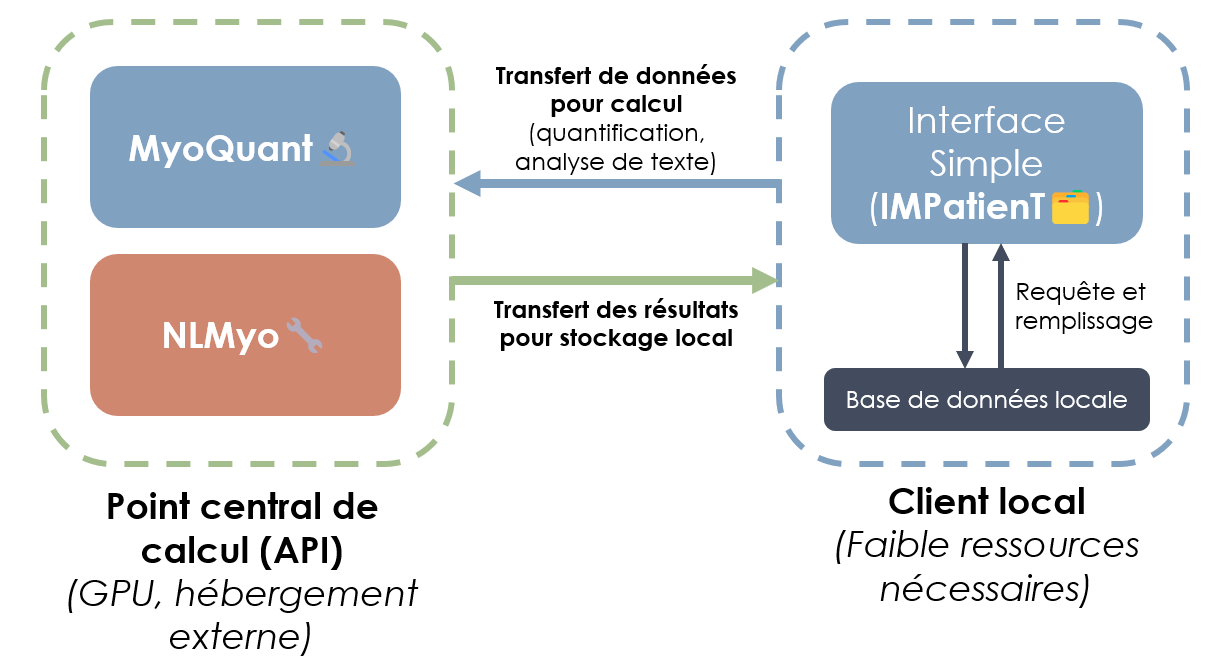
\includegraphics[width=1\textwidth]{figures/perspective_unique.png}
 \caption[Architecture de la plateforme unique en deux parties]{\textbf{Architecture de la plateforme unique en deux parties.} Un client local (à droite) servant d'interface et hébergeant les données et un serveur de calcul distant mutualisé (à gauche) mettant à disposition les modèles IA et les ressources de calcul nécessaires.}
 \label{fig:perspective_unique}
\end{figure}

La figure \ref{fig:perspective_unique} présente l'architecture prévue pour la plateforme unifiée. Le client serait une interface simple permettant d'interagir avec une base de données hébergée localement chez l'utilisateur afin de maintenir la confidentialité et le contrôle des données. À partir de cette interface, il serait possible d'ajouter des patients et de lancer des analyses des données enregistrées (quantification d'images par \gls{myoquant}, ou analyse de texte par \gls{nlmyo}). Ces analyses de données seraient alors déléguées au point central de calcul. Ainsi le client transfèrerait uniquement les données nécessaires à l'\gls{ia} au point central de calcul, qui, quant à lui, fournirait les résultats à stocker localement au client.

Cette architecture est adaptée, car elle permet à la fois de garantir la confidentialité des données, donnant le contrôle total de leurs données aux chercheurs. Mais aussi elle permet de mutualiser les couts en ressources informatiques des modèles \gls{ia} avec un point central pour plusieurs clients, dont le déploiement et la maintenance seraient assurés par notre expertise. Au final, cette architecture adaptée en deux parties, qui intègre les trois outils présentés dans cette thèse, permet à la fois de répondre aux challenges techniques tout en facilitant l'utilisation d'\gls{ia} au service de l'analyse des données biomédicales pour les chercheurs.
